\documentclass[aspectratio=169]{beamer}
\usepackage{preamble_beamer}


\title[Стохастические дифференциальные уравнения]{Лекция 3. Стохастические дифференциальные уравнения} % The short title appears at the bottom of every slide, the full title is only on the title page


\begin{document}

\begin{frame}
\titlepage 
\end{frame}

\begin{frame}{Рекап прошлой лекции}
    \begin{itemize}
        \item Броуновское движение как предел случайного блуждания. Аксиоматические определения, основные свойства.
        \item Основные понятия стох. анализа: непрерывность и дифференцируемость в с.к., полная и квадратичная вариация процесса.
        \item Интеграл Ито. Мартингальность, изометрия Ито. Отличия от интеграла Римана.
        \item Процессы Ито.
        \item Формула Ито, таблица умножения стох. дифференциалов. 
    \end{itemize}
\end{frame}

\begin{frame}{Стохастические диф. уравнения}
    Интегральная запись:
    $$
        X_t = X_0 + \int_0^t \mu(s, X_s) ds + \int_0^t \sigma(s, X_s) dB_s
    $$
    Дифференциальная запись:
    $$
        \begin{cases}
            d X_t = \mu(t, X_t) dt + \sigma(t, X_t) dB_t \\
            X_0 = x_0
        \end{cases}
    $$
\end{frame}

\begin{frame}{Пример. Броуновское движение со сносом}
    $$
        dX_t = \mu dt + \sigma dB_t 
    $$
     
    $$
        X_t = X_0 + \mu t + \sigma B_t
    $$
    \makebox[\textwidth]{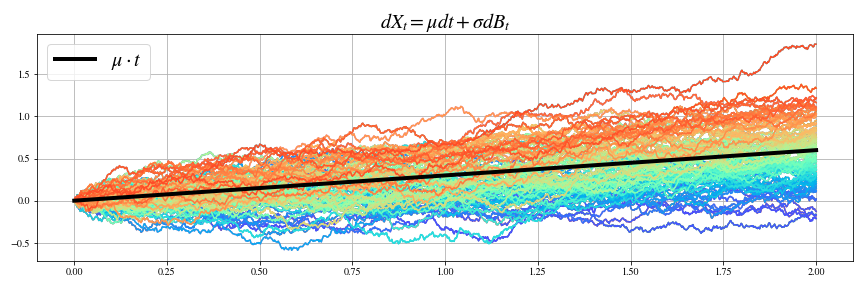
\includegraphics[width=1.0\textwidth]{2_figs/BM with drift.png}}
\end{frame}

\begin{frame}{Пример. Геометрическое броуновское движение}
    $$\begin{cases}
            dX_t = X_t \left( \mu dt + \sigma dB_t \right) \\
            X_0 = 1
    \end{cases}$$
      Рассмотрим детерменированное уравнение:
    $$
        dX_t = X_t \mu dt \to X_t = e^{\mu t}
    $$
     
    Замена переменных:
    $$X_t = e^{Y_t} \longrightarrow  Y_t = \log X_t$$
      
    $$d Y_t = \dfrac{d X_t}{X_t} - \dfrac{1}{2} \dfrac{(dX_t)^2}{X_t^2} =\left( \mu - \dfrac{1}{2}\sigma^2 \right) dt + \sigma dB_t$$
     
    $$X_t = \exp\left[ \left( \mu - \dfrac{1}{2}\sigma^2 \right) t + \sigma B_t \right]$$
\end{frame}

\begin{frame}{Пример. Геометрическое броуновское движение}
    $$X_t = \exp\left[ \left( \mu - \dfrac{1}{2}\sigma^2 \right) t + \sigma B_t \right]$$
    
    $$
        \mathbb{E} X_t =   \exp \left[ \left( \mu - \dfrac{1}{2}\sigma^2 \right) t \right] \mathbb{E} \exp \left[
            \sigma B_t
        \right] = X_0 e^{\mu t}
    $$
    \makebox[\textwidth]{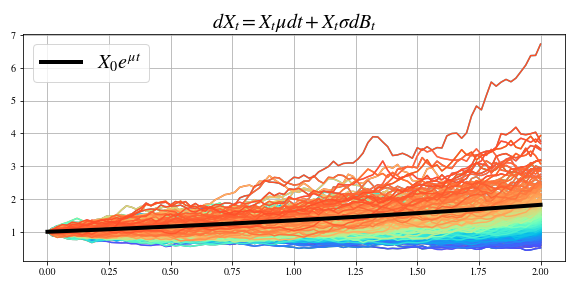
\includegraphics[width=1.0\textwidth]{2_figs/GBM.png}}
\end{frame}

\begin{frame}{Пример. Процесс Орнштейна-Уленбека}
    $$
        d X_t = \alpha (\theta - X_t) dt + \sigma dB_t
    $$

    \makebox[\textwidth]{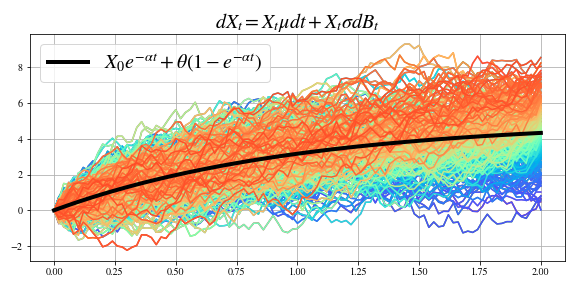
\includegraphics[width=1\textwidth]{2_figs/OU.png}}
\end{frame}

\begin{frame}{Пример. Броуновский мост}
    \begin{block}{Определение}
        Броуновский мост это гауссовский процесс $X_t$, $t\in[0, 1]$:
        \begin{itemize}
            \item $\E X_t = 0$
            \item $\mathrm{cov}(X_t, X_s) = s\cdot (1 - t), \; s \leq t$
        \end{itemize}
        Если $B_t$ -- БД, то $X_t = B_t - t \cdot B_1$ -- броуновский мост.
    \end{block}
    Броуновский мост как процесс Ито
    $$
        d X_t = a(t) X_t dt + \sigma dB_t
    $$
    \makebox[\textwidth]{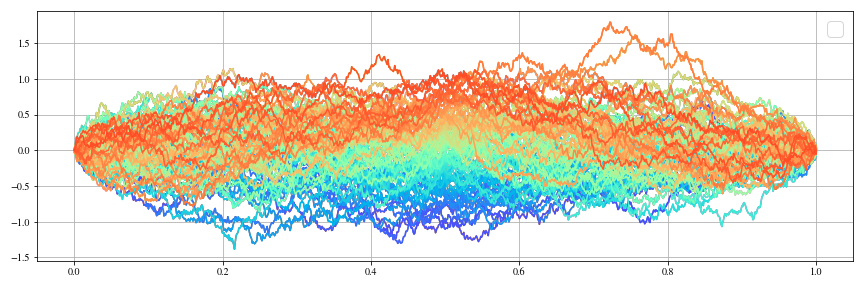
\includegraphics[width=0.6\textwidth]{2_figs/BrownianBridge.png}}
\end{frame}

\begin{frame}{Теорема существования}
    Пусть задано стохастическое дифф. уравнение:
    $$
        dX_t = \mu(t, X_t) dt + \sigma(t, X_t) dB_t
    $$
    \begin{block}{Теорема}
        Пусть 
        \begin{itemize}
            \item $|\mu(t, x) - \mu(t, y)| \leq K |x - y|$
            \item $|\sigma(t, x) - \sigma(t, y)| \leq K |x - y|$
            \item $|\mu(t, x)| + |\sigma(t, y)| \leq K (1 + |x|)$
        \end{itemize}

        Тогда $\exists !$ решение СДУ $(X_t)_{t\geq 0}$, причем:
        \begin{itemize}
            \item $(X_t)_{t\geq 0}$ адаптированный к $(\F_t)_{t\geq0}$ процесс,
            \item $(X_t)_{t\geq 0}$ имеет непрерывные траектории,
            \item $(X_t)_{t\geq 0}$ -- марковский процесс
        \end{itemize}
    \end{block}
\end{frame}

\begin{frame}{Численное решение СДУ: схема Эйлера}
    
    \begin{itemize}
        \item Пусть $0 = t_0 < t_1 < \ldots < t_n = t$ -- разбиение $[0, t]$
        \item Схема Эйлера:
        $$
            \hat{X}_{t_{k + 1}} = \hat{X}_{t_k} + \mu(t_k, \hat{X}_{t_k}) \Delta t_k + \sigma(t_k, \hat{X}_{t_k}) \sqrt{\Delta t_k} \xi_k
        $$
        где $\xi_k \sim \mathcal{N}(0, 1)$ -- i.i.d.
        \item При $\Delta t_k \to 0$ дискретный процесс $\hat{X}_{t_k} \to X_t$.
        \item Дискретная марковская цепь:
        $$
            \PP(\hat{X}_{t_{k + 1}} \in A | \F_{t_k}) = 
            \PP(\hat{X}_{t_{k + 1}} \in A | X_{t_k}) =
            \mathcal{N}\left(\hat{X}_{t_k} + \mu(t_k, \hat{X}_{t_k}) \Delta t_k, \sigma^2(t_k, \hat{X}_{t_k}) \Delta t_k\right)
        $$
    \end{itemize}

\end{frame}
% \section{}

\begin{frame}{Формула Феймана-Каца: мотивировка}
    \begin{itemize}
        \item Процесс цены $X_t$:
        $$
            dX_t = \mu(t, X_t) dt + \sigma(t, X_t) dB_t
        $$
        \item Случайная выплата, зависящая от цены $X_T$: $Y_T = \Phi(X_T)$.
        \item Ожидание выплаты в момент $t$:
        $$
            Y_t = \E \left[ \Phi(X_T) | \F_t \right]
        $$
        \item В силу марковости:
        $$
            Y_t = \E \left[ \Phi(X_T) | \F_t \right] = \E \left[ \Phi(X_T) | X_t \right] = f(t, X_t)
        $$для некоторой функции $f : \R^+\times \R \to \R$
    \end{itemize}

    \begin{block}{Постановка задачи}
        Найти функцию $f(t,x)$ такую, что:
        $$
            f(t, x) = \E[\Phi(X_T) | X_t=x]
        $$
    \end{block}

\end{frame}

\begin{frame}{Формула Феймана-Каца}
    \begin{itemize}
        \item Предположим, что $f(t, x)$ гладкая, тогда по формуле Ито:
        $$
            dY_t = \mu^Y_t dt + \sigma^Y_t dB_t,
        $$где \noident
        \begin{align*}
            &\mu^Y_t = f_t(t, X_t) + f_x(t, X_t) \mu(t, X_t) + 0.5 \cdot f_{xx}(t, X_t) \sigma^2(t,X_t) \\
            &\sigma_t^Y = f_x(t, X_t) \sigma^2(t, X_t) 
        \end{align*}
        \item $Y_t$ -- мартингал Леви, поэтому $\mu^Y_t = 0$, откуда:\noident
        \begin{align*}
            &f_t(t, x) + f_x(t, x) \mu(t, x) + 0.5 \cdot f_{xx}(t, x) \sigma^2(t, x) = 0 \\
            &f(T, x) = \Phi(x)
        \end{align*}
    \end{itemize}
\end{frame}

\begin{frame}{Формула Феймана-Каца}
    Пусть $X_t$ удовлетворяет СДУ $dX_t = \mu(t, X_t) dt + \sigma(t, X_t) dB_t$. 
    \begin{block}{Теорема}
    \begin{itemize}
        \item Пусть $f(t, x)$ удовлетворяет УРЧП:
        \begin{align*}
            &f_t(t, x) + f_x(t, x) \mu(t, x) + 0.5 \cdot f_{xx}(t, x) \sigma^2(t, x) = 0 \\
            &f(T, x) = \Phi(x)
        \end{align*} Тогда:
        $$
            Y_t = \E[\Phi(X_T) | \F_t] = f(t, X_t)
        $$

        \item Пусть $f(t, x) = \E[\Phi(X_T) | X_t = x]$. Тогда $f(t, x)$ удовлетворяет уравнению:
        \begin{align*}
            &f_t(t, x) + f_x(t, x) \mu(t, x) + 0.5 \cdot f_{xx}(t, x) \sigma^2(t, x) = 0 \\
            &f(T, x) = \Phi(x)
        \end{align*}
    \end{itemize}
    \end{block}
\end{frame}

\begin{frame}{Пример}
    Решить УРЧП:
    \begin{align*}
        &f_t(t, x) + 0.5 \cdot f_{xx}(t, x)  = 0 \\
        &f(T, x) = x^2
    \end{align*}

    \pause
    \begin{itemize}
        \item $\mu(t, x) = 0, \; \sigma(t, x) = 1 \to X_t = B_t$. 

        \item По формуле Феймана-Каца:
        $$
            f(t, x) = \E[B_T^2 | B_t = x] = \E[ (x + (B_T-B_t))^2 | B_t = x ] = \E(x+\xi)^2
        $$где $\xi \sim N(0, T-t)$.

        \item Отсюда:
        $$
            f(t, x) = x^2 + (T-t)
        $$
    \end{itemize}
\end{frame}


\begin{frame}{Инфинитезимальный оператор}
    Пусть задано стохастическое дифф. уравнение:
    $$
        dX_t = \mu(t, X_t) dt + \sigma(t, X_t) dW_t
    $$
    \begin{block}{Определение}
    Дифференциальный оператор $A$, действующий на гладкие функции $h(x)$ следующим образом:
    $$
        Ah(x) = \mu(t, x) \dfrac{\partial h}{\partial x}(x) + \dfrac{1}{2}\sigma^2(t, x) \dfrac{\partial^2 h}{\partial x^2}(x)
    $$ называется инфинитезимальным оператором.        
    \end{block}

    Формулу Ито можно записать как:
    $$
        df(t, X_t)=\left(\dfrac{\partial f}{\partial t}+Af\right)dt +\dfrac{\partial f}{\partial x}\sigma dW_t
    $$

\end{frame}

\begin{frame}{Формула Феймана-Каца}
    Пусть $X_t$ удовлетворяет СДУ $dX_t = \mu(t, X_t) dt + \sigma(t, X_t) dB_t$, \\ $A$ -- инфинитезимальный оператор процесса $X_t$. 
    \begin{block}{Теорема}
    \begin{itemize}
        \item Пусть $f(t, x)$ удовлетворяет УРЧП:
        \begin{align*}
            &f_t(t, x) + Af = 0 \\
            &f(T, x) = \Phi(x)
        \end{align*} Тогда:
        $$
            Y_t = \E[\Phi(X_T) | \F_t] = f(t, X_t)
        $$

        \item Пусть $f(t, x) = \E[\Phi(X_T) | X_t = x]$. Тогда $f(t, x)$ удовлетворяет уравнению:
        \begin{align*}
            &f_t(t, x) + Af = 0 \\
            &f(T, x) = \Phi(x)
        \end{align*}
    \end{itemize}
    \end{block}
\end{frame}

\begin{frame}{Обратное уравнение Колмогорова}
    \begin{itemize}
        \item Пусть $\Phi(x) = \delta(x-y)$ -- дельта-функция. 
        \item Переходная плотность $$p(t, x; T, y) = \E[\Phi(X_T) | X_t = x]$$
        \item $p(t, x; T, y) dy = \PP(X_T \in [y, y + dy] | X_t = x)$.
        \item \textbf{Обратное уравнение Колмогорова}:
        \begin{align*}
            &\dfrac{\partial p}{\partial t}(t, x; T, y) + Ap(t, x; T, y) = 0 \\
            &p(t, x; T, y) \to \delta(x - y) \text{ при } t \to T
        \end{align*}
    \end{itemize}
\end{frame}

\begin{frame}{Дискретная модель}
    \begin{itemize}
        \item Однородная марковская цепь. Переходные веростноятс:
        $$
            \pi(x, y) = \PP (X_{t + 1} = y | X_{t} = x)
        $$
        \item Динамика функций:
        $$
            f(t, x) = \E (\Phi(X_T) | X_t = x)
        $$
        $$
            f(t, x) = \E (f(t+1, X_{t+1}) | X_t = x) = \sum_y \pi(x, y) f(t+1, y)
        $$
        \item В матричной форме:
        $$
            \vec{f}_t = \pi \vec{f}_{t+1}
        $$

        \item Динамика маргинального распределения:
        $$
            p_t(x) = \PP (X_t = x) = \sum_y \PP (X_t = x | X_{t-1} = y) \PP(X_{t-1}=y) = \sum_y \pi(y, x) p_{t-1}(y)
        $$
        \item В матричной форме:
        $$
            \vec{p}_t = \pi^{\top} \vec{p}_{t-1}
        $$
    \end{itemize}
\end{frame}

\begin{frame}{Прямое уравнение Колмогорова}
    \begin{itemize}
    \only<1>{
        \item Пусть $X_t$ удовлетворяет СДУ: 
        $$dX_t = \mu(t, X_t) dt + \sigma(t, X_t) dB_t$$
        \item Инфинитезимальный оператор процесса $X_t$:
        $$
            Ah(x) = \mu(t, x) \dfrac{\partial h}{\partial x}(x) + \dfrac{1}{2}\sigma^2(t, x) \dfrac{\partial^2 h}{\partial x^2}(x)
        $$
        \item $p(s, y)$ -- плотность распределения с.в. $X_s$ в точке $y$
        \item $h(s, y)$ -- произвольная гладкая финитная функция, $0\leq s \leq t$.
        \item Формула Ито:
        $$
            h(t, X_t) = h(0, X_0) + \int_0^t \left(\dfrac{\partial h}{\partial s} + Ah\right)(s, X_s) ds + 
            \int_0^t \dfrac{\partial h}{\partial x}(s, X_s) dB_s
        $$
        \item В силу финитности $h(t, X_t) = h(0, X_0) = 0$.}
    \only<2>{ 
        \item     Возьмем слева и справа мат. ожидание:
        $$
            \E\int_0^t \left(\dfrac{\partial h}{\partial s} + Ah\right)(s, X_s) ds = 0 
        $$

        \item     Поменяем местами интегрирование и мат. ожидание:
        $$
            \int_0^t  ds \E \left(\dfrac{\partial h}{\partial s} + Ah\right)(s, X_s) = 0 
        $$

        \item Запишем мат. ожидание как интеграл по плотности:
        $$
            \int_0^t ds \int_{\R} p(s, y) \left(\dfrac{\partial h}{\partial s} + Ah\right)(s, y) = 0
        $$}

    \only<3>{\item Проинтегрируем по частям:
        $$
            \int_0^t ds \int_{\R} h(s, y) \left(-\dfrac{\partial p}{\partial s} + A^*p\right)(s, y) = 0
        $$где сопряженный оператор $A^*$:
        $$A^*h = -\dfrac{\partial \left(\mu(t, x)\cdot h(x)\right)}{\partial x} + \dfrac{1}{2} \dfrac{\partial^2 \left(\sigma^2(t, x) h(x)\right)}{\partial x^2}$$
        
        \item В силу произвольности $h(s, y)$ получим \textbf{прямое уравнение Колмогорова}:
        $$
            -\dfrac{\partial p}{\partial s}(s, y) + A^*p(s, y) = 0
        $$}
    \end{itemize}
\end{frame}

\begin{frame}{Прямое уравнение Колмогорова}
    Пусть $X_t$ удовлетворяет СДУ $dX_t = \mu(t, X_t) dt + \sigma(t, X_t) dB_t, X_0 = x_0 \in \R$, 
    \\ $A$ -- инфинитезимальный оператор процесса $X_t$, $A^*$ -- его сопряженный.
    \begin{block}{Теорема}
        Пусть $p(s, y)$ -- плотность распределения с.в. $X_s$ в точке $y$. Тогда $p(s, y)$ удовлетворяет уравнению:
        $$
            -\dfrac{\partial p}{\partial s}(s, y) + A^*p(s, y) = 0
        $$с начальными условиями:
        $$
            p(s, y) \to \delta(y - X_0), \; s \to +0
        $$
    \end{block}
\end{frame}

\begin{frame}{Уравнение Колмогорова и формула Феймана-Каца}
    \begin{itemize}
        \item Уравнение Колмогорова: динамика плотности вперёд во времени
        \item Уравнение (формула) Феймана-Каца: динамика УМО назад во времени 
    \end{itemize}
    \makebox[\textwidth]{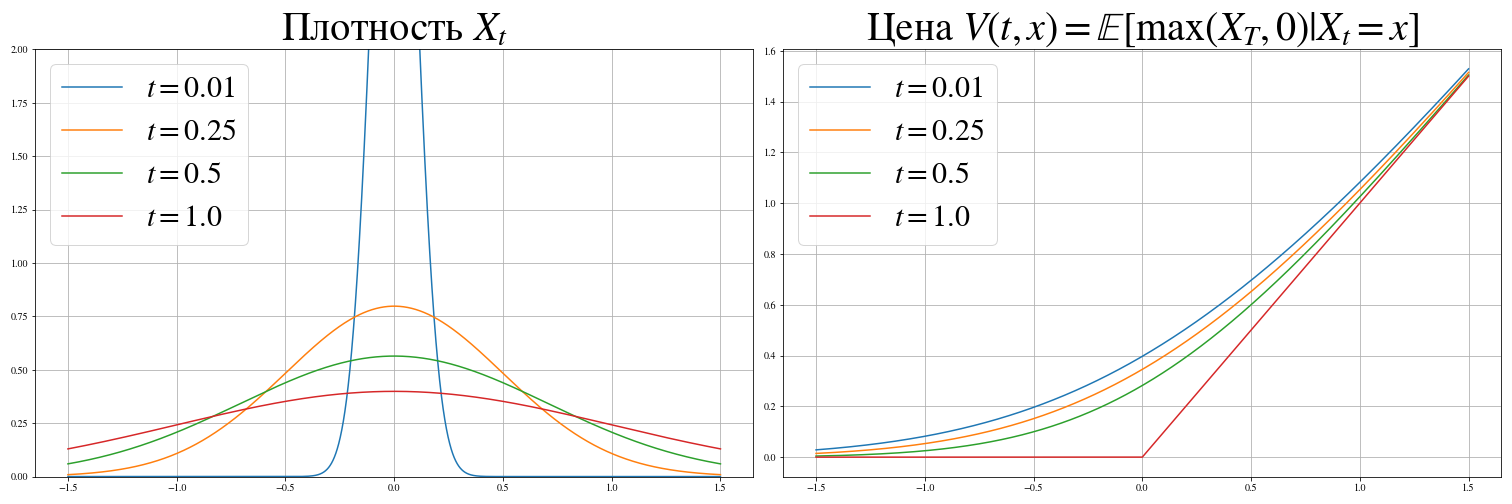
\includegraphics[width=1.0\textwidth]{3_figs/динамика плотности и цены.png}}
\end{frame}

\begin{frame}{Прямое уравнение Колмогорова: пример}
    \begin{itemize}
       \item $X_t = B_t$. Прямое уравнение Колмогорова на плотность $p(t, x)$:
        \begin{align*}
            &p_t = 0.5 p_{xx} \\
            &p(0, x) = \delta(x-x_0)
        \end{align*}

        \item Уравнение на характеристическую функцию $\phi(t, k) = \int_{\R} p(t, x) e^{ikx} dx$:
        \begin{align*}
            &\phi_t = -0.5 k^2 \phi \\
            &\phi(0, k) = e^{ikx_0}
        \end{align*}
        
        \item Решение: 
        $$
            \phi(t, k) = \exp(ikx_0-\dfrac{t k^2}{2})
        $$ 

        \item Восстановление плотности:
        $$
            p(t, x) = \dfrac{1}{2\pi} \int_{\R} \phi(t, k) e^{-ikx} dk = \dfrac{1}{\sqrt{2\pi t}} \exp(-\dfrac{(x-x_0)^2}{2t})
        $$
    \end{itemize}
\end{frame}

\begin{frame}{Приложения}

\begin{center}
\Large Приложения
\end{center}

\end{frame}

\begin{frame}{Прямое уравнение Колмогорова: пример}
    \begin{itemize}
        \only<1>{\item Пусть $X_t = B_t$
        \item $\mu(t, x) = 0, \; \sigma(t, x) = 1$
        \item $A = A^* = \frac{1}{2} \frac{\partial^2}{\partial x^2}$
        \item Обратное уравнение Колмогорова на плотность $p(t, x)$:
        $$
            p_t = \dfrac{1}{2} p_{xx}
        $$
        \item Ищем решение в автомодельном виде: $p(t, x) = \dfrac{1}{\sqrt{t}} g(\xi)$ где $\xi = \dfrac{x}{\sqrt{t}}$.
        \item $p_x = \dfrac{g'}{t}, p_{xx} = \dfrac{g''}{t^{3/2}}$
        \item $p_t = -g'\dfrac{x}{2t} - g \dfrac{1}{2t^{3/2}}= -\dfrac{\left( g' \xi + g \right)}{2t^{3/2}} $
        }
        \only<1-2>{\item Подставляем в уравнение:
        $$
            -\dfrac{\left( g' \xi + g \right)}{2t^{3/2}}  = \dfrac{1}{2} \dfrac{g''}{t^{3/2}}
        $$}
        \only<2>{
        \item Переносим всё в одну сторону:
        \begin{align*}
            &g'' + g'\xi + g = 0 \\
            &g'' + (g\xi)' = 0\\
            &g' + g\xi = 0
        \end{align*}
        \item Итого: 
        $$
            g = C\exp\left(-\dfrac{\xi^2}{2}\right)
        $$
        \item Из условий нормировки:
        $$
            p(t, x) = \dfrac{1}{\sqrt{2\pi t}} \exp\left(-\dfrac{x^2}{2t}\right)
        $$}
    \end{itemize}
\end{frame}

\begin{frame}{Уравнение Колмогорова: численное решение}
    \begin{itemize}
        \only<1>{\item Введём сетку по времени и по пространству
        $$
            t_n = n \cdot \Delta, \; x_m = m \cdot h
        $$
        \item Введём сеточные функции
        $$
            p^n_m = p(t_n, x_m)
        $$
        \item Аппроксимуруем производные:
        $$
            p_t(t_n, x_m) \approx \dfrac{p^{n+1}_m - p^n_m}{\Delta}, \; p_{xx}(t_n, x_m) \approx \dfrac{p^n_{m+1} - 2p^n_m + p^n_{m-1}}{h^2}
        $$
        \item Уравнение:
        $$
            \dfrac{p^{n+1}_m - p^n_m}{\Delta} = \frac{\sigma^2}{2 h^2} \left( p^n_{m+1} - 2p^n_m + p^n_{m-1} \right)
        $$}
        \only<1-2>{\item Выразим $p^{n+1}_{m}$:
        $$
            p^{n+1}_{m} = p^n_m + \frac{\Delta \sigma^2}{2h^2}\left( p^n_{m+1} - 2p^n_m + p^n_{m-1} \right)
        $$}
        \only<2>{\item Пусть $h^2 = \Delta \sigma^2$. 
        $$
            p^{n+1}_{m} = \dfrac{p^n_{m+1} + p^n_{m-1}}{2}
        $$}
    \end{itemize}
    \only<2>{
        \makebox[\textwidth]{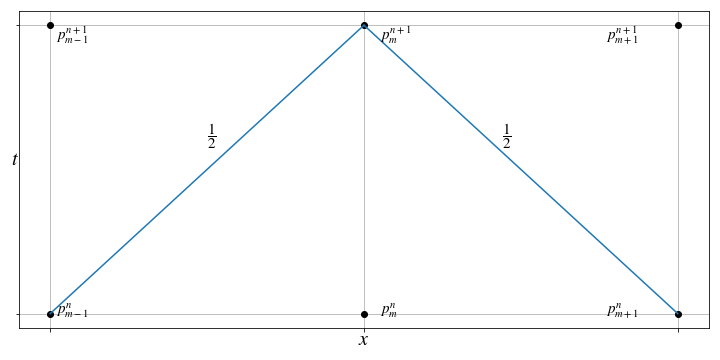
\includegraphics[width=0.6\textwidth]{3_figs/разностная схема.png}}
    }
\end{frame}

% \begin{frame}{Двойственность}
%     \begin{itemize}
%         \item Введём оператор условного мат. ожидания:
%         $$
%             (T_t \phi)(x) = \E \left[ \phi(X_t) | X_0 = x \right]
%         $$
%         \item $T_t : C(\R) \to C(\R)$.
%         \item Сопряженное пространство: пространство мер. Скалярное произведение:
        
%         $$\langle \phi, \rho \rangle = \int_{\R} \phi(x) \rho(x) dx = \E^{x \sim \rho} \phi(x)$$
        
%         \item Сопряженный оператор $T_t^*$:
%         $$\langle \phi, T_t^* \rho \rangle := \langle T_t \phi, \rho \rangle$$

%         $$\E^{x \sim T_t^* \rho} \phi(x) = \E^{x \sim \rho} (T_t \phi)(x)
%         = \E^{x \sim \rho} \E \left[ \phi(X_t) | X_0 = x \right] = \E \phi(X_t)$$

%         \item $T_t^*$ -- оператор переходной вероятности: 
%         $$
%             (T_t^* \rho)(x) = \int_{\R} \rho(x_0) \PP_t(x | x_0) dx_0
%         $$где $\PP(x | x_0) dx = \PP (X_t \in [x, x + dx] | x_0)$
%     \end{itemize}
% \end{frame}


% \begin{frame}
%     \begin{itemize}
%         \item $P(x_0)$ -- начальная плотность
%         \item Динамика плотности задаётся оператором $T_t$:
%         $$
%             P(x_t) = T_t P(x_0) = \int_{\R} P(x_t | x_0) P(x_0) dx_0
%         $$
%         \item Обратная динамика на функции:
%         $$
%             \phi(x_0) = \E \left[ \phi(x_t) | x_0 \right]
%         $$
%         $$
%             \E \phi(x_0) = \E \E \left[ \phi(x_t) | x_0 \right] = \E \phi(x_t)
%         $$
        
%         \item Двойственность: 
%         $$
%             \langle P(x_0), \phi(x_0) \rangle
%             = \langle P(x_t), \phi(x_t)\rangle
%             = \langle T_t P(x_0), \phi(x_t)\rangle
%             = \langle P(x_0), (T_t^* \phi)(x_0)\rangle
%         $$  
%         \item Сопряженный оператор:
%         $$
%             (T_t^* \phi)(x_0) = \E \left[ \phi(x_t) | x_0 \right]
%         $$
%     \end{itemize}
% \end{frame}



% \begin{frame}{Приложения}
%     Приложения
% \end{frame}


% \begin{frame}{Сильное и слабое решение}
%     Пусть $(\Omega, \F, \mathbb{P})$ -- вероятностное пространство, $(W_t)_{t\geq0}$ -- броуновское движение, $(\F_t)_{t\geq 0}$ -- естественная фильтрация. Пусть задано стохастическое дифф. уравнение:
%     $$
%         dX_t = \mu(t, X_t) dt + \sigma(t, X_t) dW_t
%     $$
%     \begin{block}{Определение}
%         Процесс $X_t$, определённый на том же вероятностном пространстве и обращающий уравнение в тождество называется \textbf{сильным} решением СДУ.
%     \end{block}
%     \begin{block}{Определение}
%         Пара из вероятностного пространства $(\tilde{\Omega}, \tilde{\F}, \tilde{\mathbb{P}})$ и процесса $\tilde{X}_t$ называется слабым решением СДУ, если выполнено:
%         $$d\tilde{X}_t = \mu(t, \tilde{X}_t) dt + \sigma(t, \tilde{X}_t) d\tilde{W}_t$$где $(\tilde{W}_t)_{t\geq 0}$ -- броуновское движение на новом вероятностном пространстве.
%     \end{block}
% \end{frame}

% \begin{frame}{Сильное и слабое решение: пример}
%     СДУ 
%     $$\begin{cases}
%         dX_t = -\mathrm{sgn}(X_t)dW_t 
%         \\
%         X_0 = 0
%     \end{cases}
%     $$имеет слабое решение, но не имеет сильное.s
% \end{frame}

% \begin{frame}{Формула Феймана-Каца}
%     Рассмотрим краевую задачу на функцию $F(t, x)$:
%     $$\begin{cases}
%         \dfrac{\partial F}{\partial t}+AF = 0 \\
%         F(T, x) = \Phi(x)
%     \end{cases}
%     $$
%     Пусть $(X_u)_{u \geq t}$ удовлетворяет СДУ     $$
%         \begin{cases}
%             dX_u = \mu(u, X_u) du + \sigma(u, X_u) dW_u
%             \\
%             X_t = x
%         \end{cases}
%     $$

%     Рассмотрим процесс $Y_u = F(u, X_u)$. По формуле Ито:
%     $$
%         Y_T = Y_t + \int_t^T \left[\dfrac{\partial F}{\partial u}+AF\right]du + \int_t^T \sigma(u, X_u) \dfrac{\partial F}{\partial x} dW_u
%     $$

%     Первый интеграл равен нулю, второй является мартингалом, откуда:
%     $$
%         Y_t = \E \left[ Y_T | \F_t\right] \to F(t, x) = \E \left[ \Phi(X_T) | \F_t\right] = \E \left[ \Phi(X_T) | X_t=x\right] 
%     $$
% \end{frame}

% \begin{frame}{Формула Феймана-Каца}
%     \begin{block}{Утверждение}
%     \begin{itemize}
%         \item         Процесс $F(t, X_t)$ мартингал относительно $(\F_t)_{t\geq0}$ тогда и только тогда, когда:
%         $$
%             \dfrac{\partial F}{\partial t}+AF = 0
%         $$
%         \item         Процесс $F(t, X_t)$ мартингал относительно $(\F_t)_{t\geq0}$ тогда и только тогда, когда:
%         $$
%             F(t,x)=\E \left[ F(T,X_T) | X_t=x\right] 
%         $$
%     \end{itemize}

%     \end{block}
% \end{frame}

% \begin{frame}{Уравнение Колмогорова}
%         Пусть задано стохастическое дифф. уравнение:
%     $$
%         dX_t = \mu(t, X_t) dt + \sigma(t, X_t) dW_t
%     $$

%     $A$ -- его инфинитезимальный оператор, $A^*$ -- сопряженный оператор. 

%     Пусть $p(s, y; t, x)$ -- переходная плотность процесса $X_t$, т.е.
%     $$
%         \mathbb{P}( X_t \in A | X_s = y) = \int_A p(s, y; t, x) dx
%     $$

%     Тогда $p(s, y; t, x)$ удовлетворяет прямому уравнению Колмогорова:
%     $$ 
%     \begin{cases}
%         \dfrac{\partial }{\partial t} p(s, y; t, x) = A^* p(s, y; t, x)\\
%         p(s, y; t, x) \to \delta(x-y) \text{ при} \; t\to s
%     \end{cases}
        
%     $$
% \end{frame}

\end{document}